\documentclass[a4paper, 11pt]{article}

%\usepackage[utf8]{inputenc}

\usepackage[top=2.5cm, left=2.5cm, right=2.5cm, bottom=3.2cm]{geometry}


% Load trebuchet in for the title and section fonts
\usepackage{fontspec}
\newfontfamily\titlefont{Trebuchet MS}

% Set up times new roman as font for text and maths
\setmainfont{XITS}

% Maths
\usepackage[fleqn]{amsmath}
\usepackage[mathrm=sym]{unicode-math}
\setmathfont{XITS Math}

% Word spacing and formatting
\usepackage[british]{babel}
\usepackage{csquotes}
\usepackage{microtype}
%\usepackage[none]{hyphenat} % prevent hyphenation to allow easy copy and paste to word template later



\usepackage{xcolor}
\usepackage{mdframed}

% Section header styling
\usepackage{sectsty}
\sectionfont{\titlefont\Large\raggedright}
\subsectionfont{\titlefont\large\raggedright}
\subsubsectionfont{\it\titlefont\normalsize\raggedright}

% Set up caption styling
\usepackage{caption}
\DeclareCaptionFormat{capfont}{\titlefont\small#1#2#3}
\captionsetup{format=capfont,font=bf,labelsep=period} 

% Hyperlinks
\usepackage[colorlinks=true, allcolors=blue]{hyperref}
\urlstyle{same}


\usepackage[detect-all]{siunitx} % SI Unit package

%\renewcommand{\labelitemi}{}
\renewcommand{\labelitemii}{$\circ$}
\renewcommand{\labelitemiii}{\footnotesize$\blacksquare$}

% Citations
\usepackage[
    backend=biber,
    bibencoding=utf8,
    sorting=nyt,
    style=apa,
    url=false, % include url in reference
    doi=false, % include doi in reference
    %sorting=none, % sorting of citations
    % autocite=superscript, % autocite becomes superscript
    maxcitenames=2, % Max names displayed when citing in text
    %maxbibnames=20, % Max number of names disaplayed in the bibliography
    giveninits=true, % Use initials
    uniquename=init
]{biblatex}
%\setlength\bibitemsep{0.1\itemsep}
\renewcommand*{\bibfont}{\small}
\addbibresource{citations.bib}

% cross-referencing
\usepackage[noabbrev, capitalise]{cleveref}

\usepackage{wrapfig}
\usepackage[]{graphicx}
\usepackage{standalone}
\usepackage{subfig}
\usepackage{tikz}

\usepackage{booktabs}
% https://tex.stackexchange.com/questions/12703/how-to-create-fixed-width-table-columns-with-text-raggedright-centered-raggedlef
\usepackage{array}
\newcolumntype{L}[1]{>{\raggedright\let\newline\\\arraybackslash\hspace{0pt}}m{#1}}
\newcolumntype{C}[1]{>{\centering\let\newline\\\arraybackslash\hspace{0pt}}m{#1}}
\newcolumntype{R}[1]{>{\raggedleft\let\newline\\\arraybackslash\hspace{0pt}}m{#1}}


\begin{document}

{
  \titlefont
  \small
  \begin{wrapfigure}{r}{0.2\textwidth}
    \raggedleft
    \vspace{-0.2cm}
    \includegraphics[width=1.8cm]{figs/design-logo.png}
  \end{wrapfigure}
  \noindent \textbf{INTERNATIONAL DESIGN CONFERENCE - DESIGN 2020}\\
  \url{https://doi.org/10.1017/dsd.2020.94}

  \vspace{2cm}

  \Large\noindent\textbf{CO-WORD GRAPHS FOR DESIGN AND MANUFACTURE KNOWLEDGE MAPPING}

  \vspace{1cm}

  \normalsize \noindent J.\ Gopsill\textsuperscript{1}, M.\ Humphrey\textsuperscript{2}, D.\ Thompson\textsuperscript{2} and E.\ Garcia\textsuperscript{2} \\[0.2cm]
  \footnotesize \noindent \textsuperscript{1}University of Bath, United Kingdom, \textsuperscript{2} National Composites Centre, United Kingdom \\[0.1cm]
  \footnotesize \noindent J.A.Gopsill@bath.ac.uk\\

  \begin{mdframed}[backgroundcolor=gray!20] 
    \normalsize \noindent \textbf{Abstract} \\
    \normalfont Design \& Manufacture Knowledge Mapping is a critical activity in medium-to-large organisations supporting many organisational activities.
    However, techniques for effective mapping of knowledge often employ interviews, consultations and appraisals.
    Although invaluable in providing expert insight, the application of such methods is inherently intrusive and resource intensive.
    This paper presents word co-occurrence graphs as a means to automatically generate knowledge maps from technical documents and validates against expert generated knowledge maps.
  \end{mdframed}

  \small \noindent \textit{Keywords: knowledge management, technology development, design informatics, graph theory}

  \vspace{0cm}
}


\section{Introduction}

Design \& Manufacture (D\&M) Knowledge Mapping is a critical activity in medium-to-large organisations.
The results support many organisational activities, such as organisational structuring, resource allocation, risk assessment and organisational strategy.
Current techniques for effective mapping of knowledge employ interviews, consultations and appraisals \parencite{jafari2009}.
Although invaluable in providing expert insight into an organisation, the application of such methods is inherently intrusive and resource intensive as they require significant time from experts to gather the necessary data and subsequent post-processing to synthesise the knowledge map.
The level of intrusion required also scales with the size of the organisation and leads to knowledge mapping activities taking months or even years to complete.
For example, the generation of a knowledge map for a timber construction company was achieved through an iterative interview and survey involving employees working on 60 timber structure projects over a six-month period \parencite{bjornfot2007}.

The mapping of knowledge becomes even more challenging when one considers Research \& Development (R\&D) organisations where new knowledge is being generated on a daily basis.
This can quickly lead to out-dated maps due to emergent terms and topics.
In addition, global organisations have R\&D facilities distributed across the world that have their own domain expertise, which poses challenges in the awareness and sharing of knowledge across transdisciplinary organisations and projects.

In these organisations, technical reporting remains the main form of knowledge capture and the advent of digital document management systems has provided an accessible store that could be automatically analysed by data mining algorithms to extract insights into the knowledge of the organisation.
However, the application of ‘off-the-shelf’ industry search technologies has been unable to effectively index and categorise these reports.
\textcite{jones2015} investigation into the search \& retrieval behaviour of employees in Airbus revealed that employees performed 1.1 M searches with many having to perform extended repeat searches to find the information they required.
This has been attributed to the lexical and logical semantic of technical reports, which is unlike websites, social media and newspapers that the search technologies have been trained on.
Thus, new approaches that are able to learn the semantics and identify domain-specific keywords is required, while also providing user-in-the-loop validation that gives employees confidence in the results being generated.

This paper contributes to the field through an adaptation of co-word analysis that enables the process to be applied to full-text documents to generate a graph of connected terminology.
It is posited, (and investigated in this paper,) that the resulting term graph properties can be used to determine whether the term should be considered a knowledge element through supervised learning where experts have labelled a sub-set of terms in the graph.
Achieving this would provide an automated method of determining emergent knowledge elements within technical document repositories.

Having identified the knowledge elements, the graph can be filtered to provide a sub-graph representing the knowledge in an organisation.
This can be partitioned to identify topics that are then mapped to designers based on authorship and document access.
The effectiveness of a community partitioning algorithm is examined and compared to partitioning by a group of discipline experts.

The paper continues by detailing the related work in the fields of knowledge mapping and co-word analysis (\cref{sec:rel}).
This is followed by the approach that adapts co-word analysis to the generation of D\&M knowledge maps that feature emergent knowledge elements (\cref{sec:km}).
To validate the approach, a scoping study to validate the approach and determine whether graph properties can be used to identify knowledge elements and subsequent partitioning into topics to the same degree of confidence as experts has been performed (\cref{sec:study}).
The findings are then discussed along with an outline of future work (\cref{sec:dis}). The paper concludes by highlighting the key findings from the scoping study (\cref{sec:con}).


\section{Related work}\label{sec:rel}

This section provides a summary of the state-of-the-art in the fields of knowledge mapping and application of co-word analysis.

\subsection{Knowledge mapping}

Knowledge mapping is a key task for organisations and a number of approaches have been developed and implemented in industry.
\textcite{jafari2009} review of knowledge mapping identified 5 techniques used in practice: Yellow Paging, Information Flow Analysis, Social Network Analysis, Process Knowledge Mapping and Functional Knowledge Mapping.
The comparison of these techniques (\cref{tbl:km}) reveals that the majority of techniques are laborious and require considerable resource from the organisation to complete.

\begin{table}[t!]
  \caption{Comparison of Knowledge Mapping techniques \parencite{jafari2009}}\label{tbl:km}
  %\scriptsize
  \fontsize{6pt}{6pt}\selectfont
  \centering
  \begin{tabular}{p{0.10\textwidth} | p{0.13\textwidth} p{0.13\textwidth} p{0.13\textwidth} p{0.13\textwidth} p{0.13\textwidth} p{0cm}}
    \toprule
    & 
    \raggedright Yellow Page & 
    \raggedright Information Flow Analysis & 
    \raggedright Social Network Analysis & 
    \raggedright Process Knowledge Mapping & 
    \raggedright Functional Knowledge Mapping & 
    \\
    \midrule
    
    \raggedright Used tools for data gathering &
    \raggedright Question and answer systems, Skill dictionary and reports &
    \raggedright Interviews, skill inventories, and extensive surveys \raggedright information flow diagram (IFD) &
    \raggedright Questionnaire, Sociogram and Graph Theory &
    \raggedright Brainstorming or conduct interviews with the process owners &
    \raggedright Survey and interview &
    \\

    \raggedright Used tools for knowledge map evaluation &
    \raggedright Skills dictionary &
    \raggedright Questionnaire, interviews and sign-out sheets &
    \raggedright InFlow, Krackplot and NetMiner &
    \raggedright -- &
    \raggedright Observations, Interviews, Internal Reports &
    \\

    \raggedright Objectives & 
    \raggedright Create transparency as to the location of knowledge in the organisation by registering individual competencies in a database or similar manner &
    \raggedright Determining who is accessing what information sources and how often &
    \raggedright Discover interaction patterns between members & 
    \raggedright Define the knowledge needed, decision milestones, the knowledge available to support a business process. Routes for access and retrieval of knowledge and Gaps between required skills and current skills. &
    \raggedright Locate knowledge sensitive areas. Identifies and characterises areas of process related critical knowledge spots. &
    \\

    \raggedright Knowledge mapping approach & 
    \raggedright Project-based & 
    \raggedright Relationship-based & 
    \raggedright Relationship-based & 
    \raggedright Process-based & 
    \raggedright Process-based &
    \\

    \raggedright Create static or dynamic map &
    \raggedright Static &
    \raggedright Static &
    \raggedright Dynamic &
    \raggedright Dynamic & 
    \raggedright Dynamic &
    \\

    \raggedright Support tacit or explicit &
    \raggedright Explicit &
    \raggedright Tacit &
    \raggedright Tacit &
    \raggedright Explicit, Tacit &
    \raggedright Explicit, Tacit &
    \\

    \bottomrule

  \end{tabular}
\end{table}


In design research, researchers have been exploring how one can overcome the laborious nature of current industry standard techniques.
For example, \textcite{dori2005} has sought to define an ontology of knowledge through extraction of explicit links in Product Data Management (PDM) systems. 
While \textcite{sarica2019,sarica2020} have investigated patent databases as a consistent and reliable source to synthesise and organise knowledge on a subject matter. They evaluated co-word analysis, part-of-speech tagging and a graph-based unsupervised extraction method. 
\textcite{schmidt2015} mapping of knowledge in student design projects utilised pre-defined knowledge elements that were then related to elements of the project and design process. 

Having generated a map, considerable research has been performed to exploit them to generate insights for industry. Example analyses include, Multi-Domain Matrices, Structural Criteria and Domain Mapping Matrices, being applied to support decision-making, project planning, strategy development and risk management \parencite{schmidt2013a,schmidt2013b,von2014}.

This brief summary of knowledge mapping highlights that industry is still using manual and laborious processes to generate knowledge maps. However, recent advancements in design research has highlighted the potential of the digital footprint, such as PDM systems and document repositories, as a data source for the generation of knowledge maps through numerical techniques. Yet, it is the validation and confidence in the results that appears to be the continuing barrier in pulling this research through into industry. In addition, the challenge of maintaining up-to-date knowledge maps where the document set is continually evolving, such as in R\&D, also remains.

\subsection{Co-word analysis}

Co-word analysis evaluates document repositories through the co-occurrence of terms. By analysing the co-occurrence of terms, a graph of connected terms (a.k.a vertices in graph theory) is generated, which enables the application of graph theory algorithms to uncover emergent structures and patterns between terms. For example, centrality measures are often used to identify the most important and influential terms, while partitioning algorithms, such as Louvain community partitioning \parencite{blondel2008,hagberg2008}, seeks to identify groups of highly connected terms within a graph, where Modularity, $Q$, is used as the objective function \parencite{newman2004,newman2006}. In the context of co-word analysis, the partitioning of terms is used to identify themes/topics.

Co-word analysis has primarily been applied in the identification of research themes within scientific communities using keywords, abstracts and summaries of documents to identify the terms of interest \parencite{ding2001,liu2014}.
It has also been used in document sets where the text has been broken down to the sentence level \parencite{le2014distributed}.
While \textcite{gopsill2015} has applied co-word analysis to small text, such as engineering e-mail, enabling the evolution of topics to be monitored and associations with requirements scope creep to be developed.
Small texts have also been of interest to \textcite{he2019} who has applied co-word analysis to synthesise concept designs from crowd-sourced ideation exercises.

\begin{figure}
    \subfloat[Matrix \parencite{gopsill2016}]{
        \includegraphics[height=3.5cm]{figs/gopsill.png}
    }
    \hfill
    \subfloat[Network \parencite{liu2014}]{
        \includegraphics[height=3.5cm]{figs/liu.png}
    }
    \hfill
    \subfloat[Strategic \parencite{jones2015subject}]{
        \includegraphics[height=3.5cm]{figs/jones.png}
    }
    \caption{Graph visualisations}
    \label{fig:graph-viz}
\end{figure}

It is not only the quantitative metrics afforded by this analytical technique but also the ability to aggregate and visualise a large corpus of information into more manageable forms for human interpretation and decision making (\cref{fig:graph-viz}).
A number of visualisation techniques have been employed and include:

\begin{itemize}
  \item Re-arranged matrices in relation to the partitioning of terms;
  \item Force-based network diagrams to reveal the connected nature of the terms; and,
  \item Strategic diagrams that show the movement of topics over time.
\end{itemize}

From this brief review of the state-of-the-art, the challenge identified is in generating accurate and detailed knowledge maps through non-manual means.
A challenge that could be overcome with an approach that moves co-word analysis away from pre-defined keywords and to whole-body text.


\section{Co-word knowledge maps}\label{sec:km}

The related work highlights the potential for co-word analysis to complement existing knowledge mapping approaches and one that would be more suitable for large organisations with vast repositories of technical reports. 
This section proposes how co-word analysis, which has typically been used on keywords and short texts, could be adapted and used to identify keywords from full-text and subsequent partitioning of these terms to identify topics of knowledge for an organisation.

\subsection{Graph generation}

The proposed process for generating co-word graphs from full-text technical engineering reports (in portable document format, PDF) follows a 4-step process:

\begin{enumerate}
  \item Document text extraction;
  \item N-gram identification;
  \item N-gram co-occurrence; and,
  \item Co-occurrence normalisation.
\end{enumerate}

These are now discussed.

Step 1 requires parsing of the PDFs and extraction of the text in UTF-8 format (Step 1).
Most technical documents are digitally curated, however if scanned, Optical Character Recognition (OCR) is required.
Regular expressions are then used to extract the year in which the report was created, authorship, and generate a list of noun-noun bi-grams contained within the main body of document (Step 2). Noun-noun bi-grams have been selected as the objective is to identify technical terms, which are often formed of multiple nouns combined together (e.g.\ carbon fibre). It is also hypothesised that the noun-noun bi-grams are the most stable feature of the lexicon and thus, suitable for knowledge mapping. The noun-noun bi-grams are then stemmed and checked against a noun stop-word list. Any bi-grams featuring a stop-word are removed and the list of bi-grams is reduced to form a unique set. The noun-noun bi-grams form the graph vertices whose frequency ($f$) is determined by their appearence in the document set and document frequency ($f_d$) determined by number of documents the term appears in.

To form the co-word edges (Step 3), indexing of the noun-noun bi-grams is performed for each document and an ordered list of bi-grams with their position indices produced. One can then loop through the list and based on a look-ahead distance, $d$, determine the bi-grams that co-occur. d or the re-appearance of the term is used as the maximum distance to prevent double counting. With the co-occurrences identified, the process either creates an edge if one does not exist or increments the weight of the edge if it does exist. \cref{lst:co} outlines the approach through a logic-flow diagram.

\begin{figure}[t]
  \centering
  \includegraphics[height=10cm]{figs/workflow.png}
  \caption{Logic-flow for determining the co-occurrence of bi-grams}\label{lst:co}
\end{figure}

Applying a look-ahead distance accounts for the likelihood of multiple topics being discussed across the sections and paragraphs of text within the technical document.
$d$ was set to 140 characters to follow examples in social media, such as twitter, where the average sentence length is 100 characters with the extra characters enabling the use of \#tags.
In the case for technical documents, the additional length in the threshold accounts for topics discussed across multiple sentences and paragraphs.

To account for variations in bi-gram frequency, normalisation is performed:
\begin{equation}
  n_{ij}=\frac{w_{ij}}{\left( f_i + f_j - 1 \right)}
\end{equation}

Where $n_{ij}$ is the normalised edge weighting and is determined by the number of times $i$ and $j$ have co-occurred ($w_{ij}$) divided by the number of co-occurrences that could have occurred ($f_i+f_j-1$).
With the co-word graph generated, one can begin to use graph properties to determine keywords and prune on the keywords to form a subgraph and hence, knowledge map.

\subsection{Graph properties for keyword identification}

The affordance of forming a co-word graph is in the provision of a number of properties that can support us in determining whether a noun-noun bi-gram accurately reflects an element of knowledge.
There is the frequency, $f$, and document frequency, $f_d$. In addition, one can look at the degree and weighted degree of the bi-gram to inform us on how connected the bi-gram is with the all other bi-grams in the graph.
Centrality measures, such as degree, eigenvector and betweenness, provide an alternative perspective on how central a bi-gram is to the graph. With these properties afforded to us, there is a question as to whether they could be used to determine noun-noun bi-grams that reflect elements of knowledge within an organisation.

\subsection{Graph partitioning for topic identification}\label{sec:topic}

To identify topics through term co-occurrence, the Louvain partitioning algorithm has been applied \parencite{blondel2008}.
The algorithm works by allocating terms to partitions with the objective of returning a partition set that produces the highest modularity score for the graph.
Modularity, $Q$, is an assessment of the quality of the matrix partition and is defined as \parencite{newman2004}:
\begin{equation}
  Q=\frac{1}{2m}\sum_{ij}\left[A_{ij}-\frac{k_ik_j}{2m}\right]\delta\left(c_i,c_j\right)
\end{equation}

Where $m=\frac{1}{2}\sum_{ij} A_{ij}$ and is the number of co-occurrences within the graph. $\delta$ is the Kronecker delta function and is 1 if a co-occurrence exists between two terms and 0 otherwise. 
$k_ik_i/2m$ is the probability that a co-occurrence may exist between two terms, where $k_i$ is the number of terms that have co-occurrences with term $i$, and $k_j$ is the number of terms that have co-occurrences with term $j$. 
And, $A_{ij}$ is the weighted co-occurrence between two terms in the graph.

To start, the algorithm assigns each term to its own partition.
The algorithm sequentially moves one file to a different partition and calculates the change in $Q$ (\cref{equ:delta-q}).
\begin{equation}
\Delta Q=\left[\frac{P_{\mathrm{in}}+k_{i,\mathrm{in}}}{2m}-\left(\frac{P_{\mathrm{tot}}+k_i}{2m}\right)^2\right]-\left[\frac{P_{\mathrm{in}}}{2m}-\left(\frac{P_{\mathrm{tot}}}{2m}\right)^2-\left(\frac{k_i}{2m}\right)^2\right]
\label{equ:delta-q}
\end{equation}

Where $P_{\mathrm{in}}$ is sum of all the normalised co-occurrence weights within the partition that term $i$ is being included in, $P_{\mathrm{tot}}$ is the sum of all the normalised co-occurrence weights to term within the partition that $i$ is being included in, $k_i$ is the co-occurrence degree of $i$, $k_{i,\mathrm{in}}$ is the sum of the normalised co-occurrence weights $i$ and other terms within the partition that $i$ is merging with.

From this, $\Delta Q_{\mathrm{max}}$ can be identified. The associated terms are then assigned to the same partition and the algorithm repeats the previous step of identifying the next term movement that will result in a further increase in modularity. If no further movement of terms achieves an increase in modularity, the algorithm terminates resulting in the partition set that gives the highest modularity score. This iterative process results in a partition set that are highly connected internally and weakly connected to one another.

Hence, it is a form of hierarchical clustering and the algorithm iterates until the modularity can no longer be increased by further aggregation of the terms. This paper uses the community API implementation of the Louvain community partitioning algorithm within the NetworkX python package\footnote{\url{https://bitbucket.org/taynaud/python-louvain/src/default/}}.


\section{Study: Achieving confidence through expert supervised learning}\label{sec:study}

To test the approach, a scoping study was performed on a subset of the National Composites Centre’s (NCC) technical report corpus. The National Composites Centre (NCC) is a world-leading R\&D centre for UK composites. Established in 2009 as a result of the UK Composite strategy, it is now part of the UK government’s CATAPULT programme of world-leading centres designed to accelerate the UK’s High-Value Manufacturing capability and drive future economic growth. The NCC currently provides R\&D support for over 40 companies.

While the full technical report repository consists of over 5,000 reports, the subset of reports used in the scoping study consisted of public-funded research projects over a four-year period. Details of the subset used is provided in~\cref{tbl:dataset}.

\begin{table}[h!]
  \center
  \caption{Dataset Statistics}
  \label{tbl:dataset}
  \footnotesize
  \begin{tabular}{*{6}r}
    \toprule
    \textbf{Year} & \textbf{\# Documents} & \textbf{$\sum$ Words} & \textbf{Mean \# Words} & \textbf{Max. \# Words} & \textbf{Min. \# Words} \\
    \midrule
    2012 & 5 & \num{31941} & \num{6388} & \num{9396} & \num{3581} \\
    2013 & 6 & \num{56201} & \num{9367} & \num{17752} & \num{2810} \\
    2014 & 7 & \num{83776} & \num{11968} & \num{20375} & \num{999} \\
    2015 & 8 & \num{68107} & \num{8513} & \num{18999} & \num{4022} \\
    \midrule
    Combined & 26 & \num{240025} & \num{9232} & \num{20375} & \num{999} \\
    \bottomrule
  \end{tabular}
\end{table}

Following the process outlined in Section 3 the co-word bi-gram graph generated featured 23,869 vertices and 130,000 edges. This graph was further pruned based on: 

\begin{itemize}
  \item low document frequency vertices ($f_d<3)$; 
  \item high document frequency vertices ($f_d>23$);
  \item low normalised edge weights ($e_w<0.1$); and,
  \item low co-occurrence frequency ($e_c<3$).
\end{itemize}

resulting in a graph featuring 834 vertices and 1,230 edges.

\begin{figure}[t!]
  \centering
  \subfloat[Vertex frequencies]{
    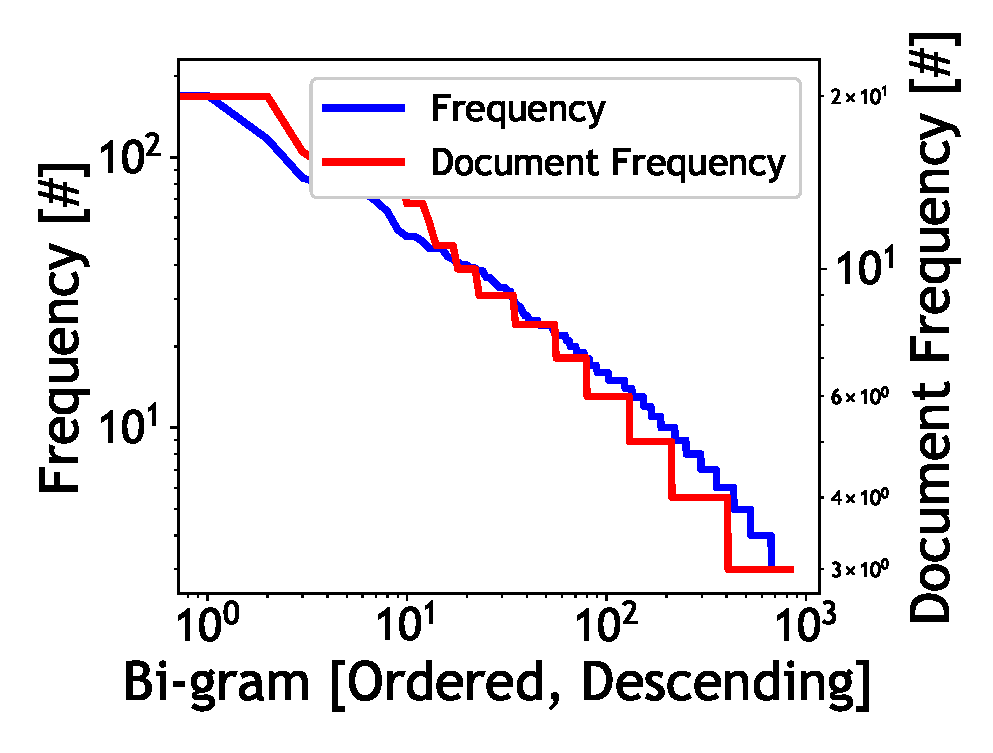
\includegraphics[width=0.45\textwidth]{figs/frequencies.eps}
  } \hfill
  \subfloat[Edge weights] {
    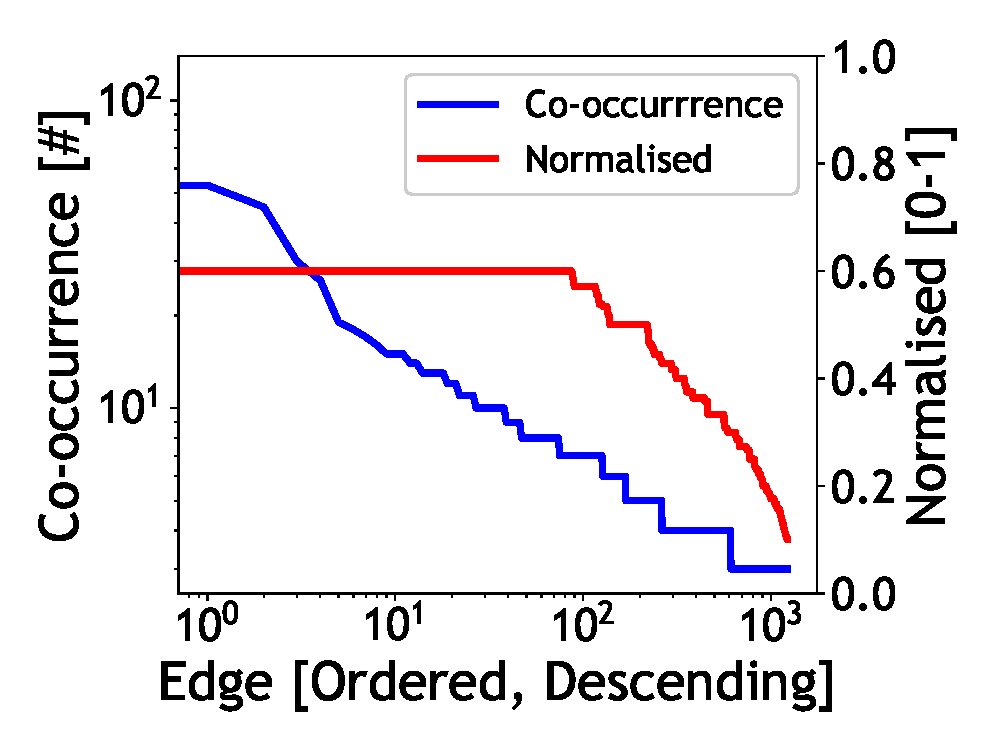
\includegraphics[width=0.45\textwidth]{figs/edge.eps}
  }
  \caption{Bi-gram co-word graph properties}\label{fig:co-word-props}
\end{figure}

\subsection{Graph properties of keywords}

With the bi-gram co-word graph pruned, the bi-grams were extracted and placed into Excel. The spreadsheet was given to a group of 5 experts who collectively determined which bi-grams were keywords representing elements of knowledge within the NCC. This resulted in a list of 104 keywords from the 354 vertices provided $\left(\sum x_k=104,\sum x_{nk}=250\right)$. 

To determine whether the graph properties could be used to differentiate between keywords and non-keywords, T-tests were performed on five properties of the graph: bi-gram frequency, bi-gram document frequency, degree, weighted degree and eigenvector centrality ($\lambda$).The results, shown in~\cref{tbl:props}, highlight a significance difference in distributions is observed for all but bi-gram frequency and document frequency. This suggests that confidence bounds based on the distributions could be placed on the graph properties to distinguish between keyword and non-keyword bi-grams. Reviewing $\bar{x}_k$ \& $\bar{x}_{nk}$ reveals that keywords appear less across the documents and have a lower degree, weighted degree and centrality.

\begin{table}[t]
  \centering
  \caption{T-test of keyword/non-keyword properties}\label{tbl:props}
  \begin{tabular}{l r r r}
    \toprule
    Property & $\bar{x}_k$ & $\bar{x}_{nk}$ & $p$ \\
    \midrule
    Frequency & 12.33 & 9.28 & $0.06$ \\
    Document Frequency & 4.30 & 4.23 & $0.82$ \\
    Degree & 1.2 & 3.01 & $<0.001$ \\
    Weighted Degree & 0.26 & 0.97 & $<0.001$ \\
    $\lambda$ Centrality & 0.00002 & 0.0091 & $<0.001$ \\
    \bottomrule
  \end{tabular}
\end{table}

\subsection{Topic identification}

With the keywords identified, the graph was pruned so that only these terms remained with the additional criteria that they needed to be connected in the graph (i.e.\ no degree of 0). This left 87 terms in the graph. The graph was subsequently partitioned using the Louvain partitioning algorithm (\cref{sec:topic}), which gave 17 partitions (10 of which are components) and $Q=0.836$ (\cref{fig:graph}). This score reveals that significant structure is present within the graph as it is generally accepted that $Q>0.3$ indicates a structure beyond that of random association \parencite{newman2004}.

To investigate the potential of co-word partitioning as a means to generate knowledge maps, the group of experts were tasked to partition the keywords into areas of knowledge (\cref{fig:card-sort}). The experts partitioned the keywords into 9 partitions.

\begin{figure}[t]

  \hfill{}
  \subfloat[Community Detection]{
    \includegraphics[height=4cm]{figs/co-word.pdf}
    \label{fig:graph}
  } 
  \hfill{}
  \subfloat[Card Sort] {
    \includegraphics[height=4cm]{figs/expert.jpg}
    \label{fig:card-sort}
  }
  \hfill{}
  
  \caption{Graph and Expert Partitioning}
\end{figure}

To compare partitions, the edit distance was applied between the two results as well as comparison with random partitioning of the keywords \parencite{deibel2005}.
Taking the Louvain partitioned set, $L$, and Expert partitioned set, $E$, the edit distance reflects the minimum number of moves that are required to convert $L$ to $E$.
This can be solved by determining the maximum number of terms not moved and can found through maximum weight matching on a bipartite graph.
A bipartite graph can be formed on partitions $L_1,\ldots,L_n and E_1,\ldots,E_n$  with an edge between $L_i$ and $E_j$ of weight $\left|L_i\cap E_j\right|$.
A complete matching between L and E is where each vertex in L is matched to a unique vertex in E. The total weight of the matching is the sum of the edge weights in the matching.
This was solved using NetworkX's implementation of the blossom and primal-dual method \parencite{galil1986}.

\begin{figure}[t!]
  \centering
  \hfill 
  \subfloat[Louvain / Expert] {
    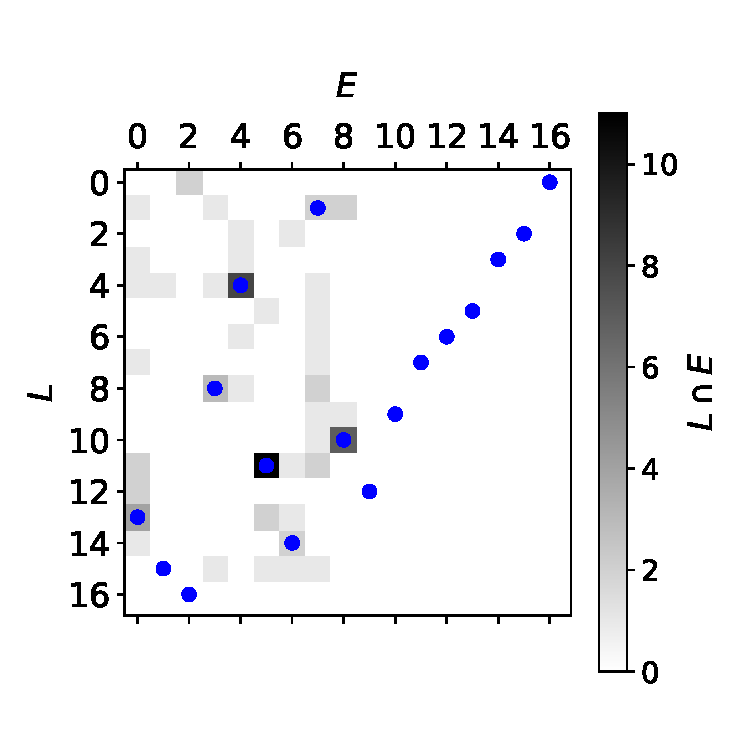
\includegraphics[width=0.31\textwidth]{figs/bipartite.eps}
  }
  \hfill 
  \subfloat[Random / Expert] {
    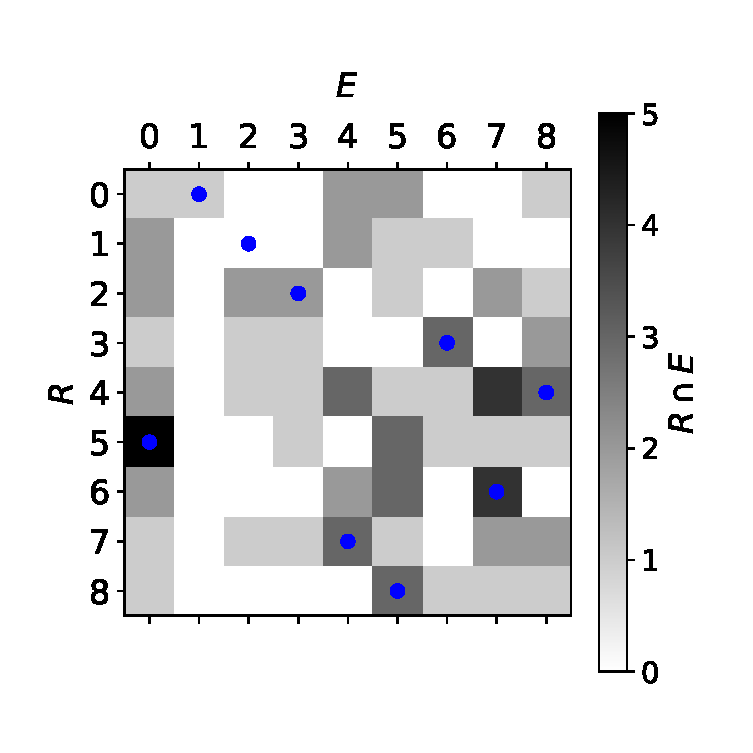
\includegraphics[width=0.31\textwidth]{figs/random.eps}
  } 
  \hfill 
  \subfloat[Random / Louvain] {
    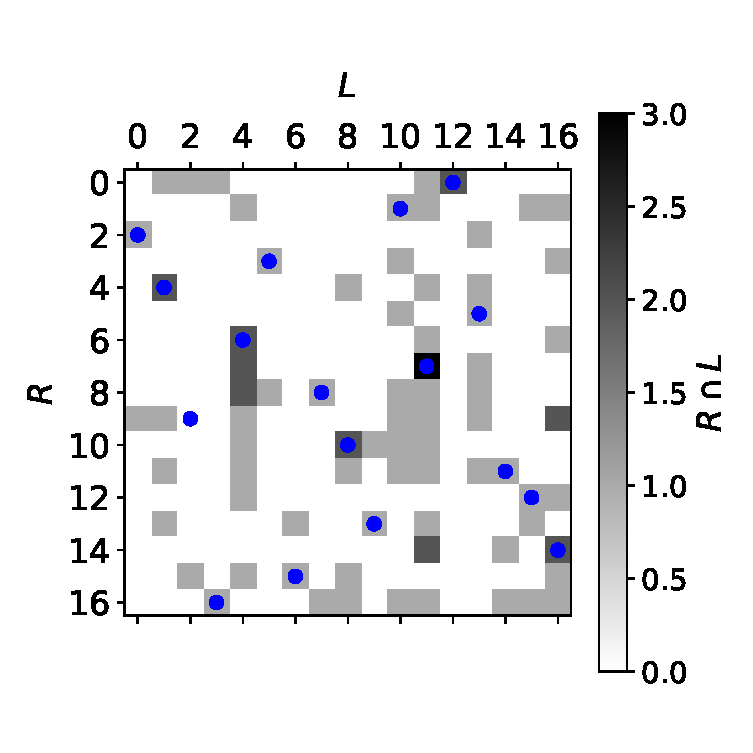
\includegraphics[width=0.31\textwidth]{figs/random-louvain.eps}
  }
  \hfill 
  \caption{Bi-partite matrices and max-weight matching}\label{fig:bipartite}
\end{figure}

\begin{table}[t!]
  \centering
  \caption{Co-word and Random Partition Comparison to Experts}\label{tbl:comparison}
  \small
  \begin{tabular}{l r r r}
    \toprule
    Measure & L & E & \\
    \midrule
    Partitions & 17 & 9 & \\
    $Q$ & 0.824 & 0.254 & \\
    \midrule
    Comparison & L-E & R-E & L-R \\
    \midrule
    Terms & 87 & 87 & 87 \\
    Maximum Weight Matching & 40 & 24 & 23 \\
    Minimum Edit Distance & 47 & 63 & 64 \\
    \bottomrule
  \end{tabular}
\end{table}

\cref{tbl:comparison} details the co-word partitioning and edit distances required to move from one partition to another. The Louvain partitioning provides the highest modularity of the graph as one would expect as it is driven by this objective function. However, the expert partitioning appears to not reflect the nature of co-occurrence with $Q=0.254$.

Looking at the minimum edit distance, Louvain and Expert is the smallest although half of the terms would still need to be re-organised to create matching groups. Both have similar edit distances to Random partitioning, which demonstrates a systematic approach to structuring the data be it through the co-occurrence of bi-grams or expert domain understanding.

\cref{fig:bipartite} provides the comparison of the topics generated by Louvain, Expert and Random with the gradient highlighting the number of same bi-grams within topics and blue dots indicating the maximum edge matching between the sets of topics. It can be seen that the contribution to the edit distance has come in the form of the additional partitions produced by Louvain, which are not captured by the expert. As the partitioning algorithm is a form of hierarchical clustering, it may be that a threshold set on the objective function would produce coarser partitions that are more in line with the expert partitioning.

\section{Discussion and future work}\label{sec:dis}

The adaption of co-word analysis to parse technical reports through the identification of bi-grams and application of a bi-gram index distance to determine co-occurrence has shown promise in identifying elements of knowledge and partitioning of knowledge elements into topics.

The potential of using graph properties to evaluate whether a bi-gram is a knowledge element has been confirmed with T-tests showing significant difference in the properties of bi-grams determined to be knowledge elements by experts. Having proved this, one can now go further in determining the thresholds and boundaries one needs to set for a bi-gram to be automatically considered a knowledge element. In addition, opportunities exist in using supervised learning where experts label a portion of the bi-gram co-word graph and allow the algorithm to propagate the labels across the graph.

The topic identification through graph partitioning revealed a structure whose edit distance is considerably less than that of random partitioning. This demonstrates that partitioning could pose as an expert in mapping knowledge although further investigation is required to determine the nature of the differences between expert and algorithmic partitioning. To achieve this, future work is planned to perform more expert knowledge map exercises to investigate the difference in knowledge maps between experts and whether the edit distance seen in this experiment is comparable to the variance observed in expert opinion.

It is also the case that the algorithm and analysis has been performed on a subset of reports. Thus, the algorithm currently lacks all the information to construct a high-fidelity knowledge map whereas the group of experts would have additional understanding of the subject matter, which they would have brought to the term partitioning exercise. This would be mitigated in subsequent studies by increasing the sample size.

The final aspect to consider is the sensitivity of the analysis due to the index distance used to determine co-occurrence as well as the size and variety of terms used in the document set. Further work could be performed to determine how the graph topology varies with these parameters. In addition, further partitioning techniques could be explored to see which best correlates with expert defined partitions, such as multicores-periphery structures \parencite{yan_luo_2019}.


\section{Conclusion}\label{sec:con}

Design \& Manufacture Knowledge Mapping continues to be a critical activity and the synthesis of maps is becoming ever more challenging as the breadth of knowledge required by organisations is increasing in order to develop products of increasing complexity. This paper has proposed and demonstrated that an adapted model of co-word analysis can complement and may even supersede the current industry standard knowledge mapping techniques. T-tests have shown that graph properties can be used to distinguish bi-grams that represent elements of knowledge and partitioning can be used to group knowledge elements into topics.

\section*{Acknowledgements}

The work reported in this paper has been undertaken as part of the UKRI NCC Researcher in Residence (EP/R513556/1) and EPSRC Trans-disciplinary Engineering (EP/R013179/1) grants.

\printbibliography[]

\end{document}